\chapter{Results and analysis}

\subsection{Canonical simulations}
%Pr 1 St 2


\begin{figure*}
\begin{center}
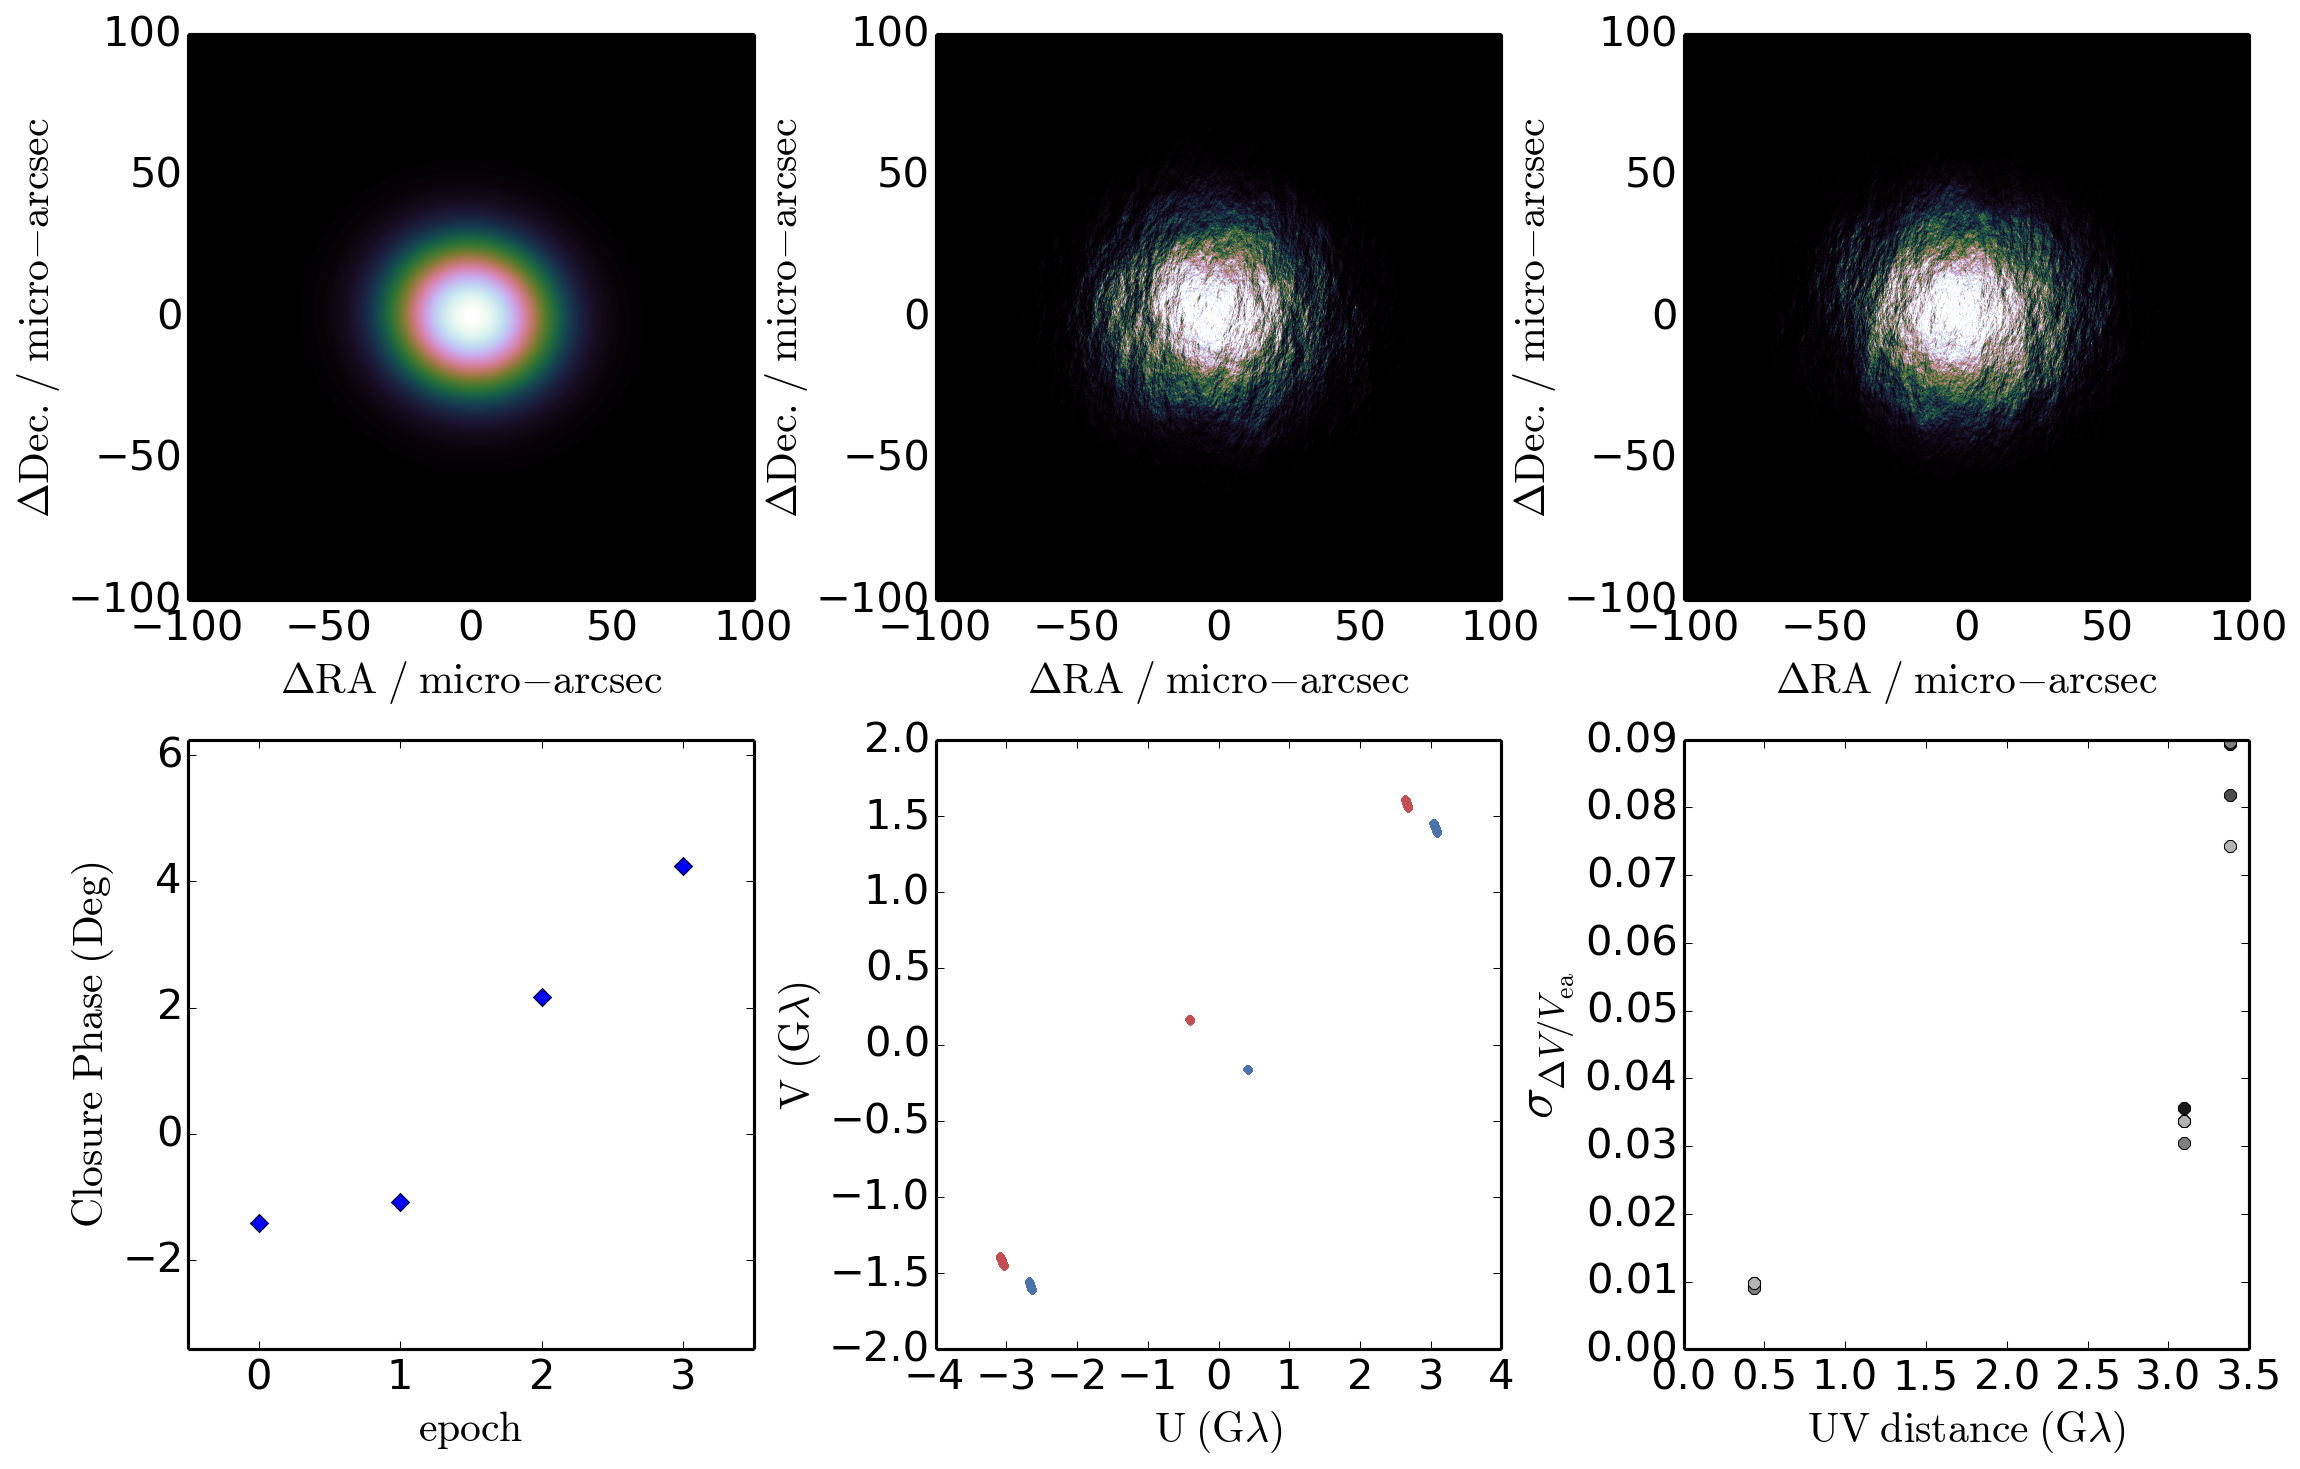
\includegraphics[width=1.8\columnwidth]{../../Images/ism}
\caption{An example simulation of ISM scattering towards Sgr~A$^{\star}$.  The top panel, left to right, shows the original $\rm FWHM = 40$~$\mu$-arcsec Gaussian {\bf (top left)}, the ISM scattered image on the first night {\bf (top middle)} and last night {\bf (top right)} of the observation respectively.  The bottom panel, left to right,  shows the evolution of the 10 minute-averaged closure phase with epoch {\bf (bottom left)}, {\sl uv}-tracks for any particular night {\bf (bottom middle)} and the visibility amplitudes $|V|$ of the unscattered (red) and scattered (grey-scale) sources as a function of {\sl uv-}distance {\bf (bottom right)}. Variations of the flux on the shortest baselines reveal total flux modulation while flux variations $\Delta |V|$ on longer baselines and non-zero closure phases track the fluctuations in refractive noise. When compared to the latest published observations of Sgr~A$^{\star}$ \protect\citep{Fish_2016}, we see that the observed and simulated closure phase variability are consistent. Furthermore, ISM scattering simulations can constrain the variability fraction associated with the screen, enabling a more robust estimation of source variability.\label{ISM_sequence}%
}
\end{center}
\end{figure*}

\begin{figure}
\begin{center}
\includegraphics[width=1.\columnwidth]{../../Images/opacity_c}
\caption{Best fit opacity (red) and sky brightness temperature (blue) line solutions at $\nu =230$~GHz as a function of precipitable water vapour (PWV) for three indicative ground pressures and temperatures which approximately represent the sites of SPT (solid), ALMA (diamond) and SMA (dashed). The legend shows the estimated input ground (pressure, temperature) parameters for each site.\label{fig:mean_atm}%
}
\end{center}
\end{figure}


\begin{figure}
\begin{center}
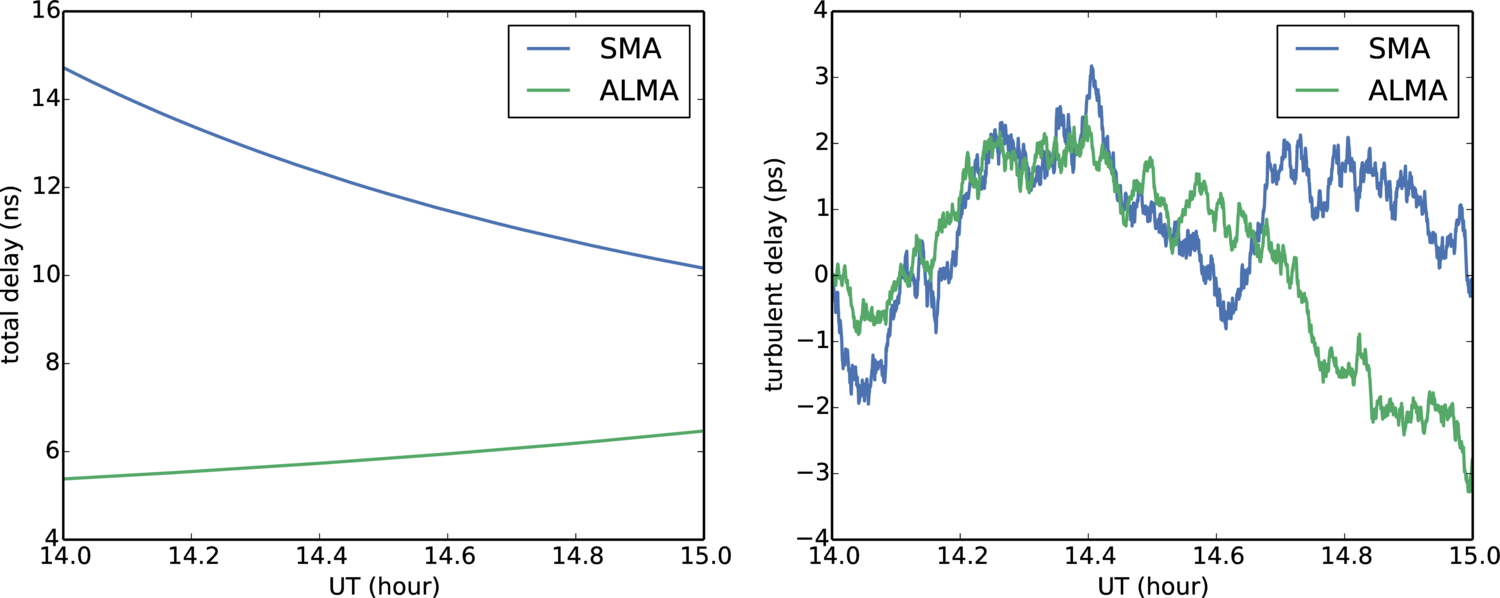
\includegraphics[width=1.\columnwidth]{../../Images/delays}
\caption{Simulation of the total delay (left) and the turbulent atmospheric delay (right) for SMA (blue) and ALMA (green) sites towards Sgr~A$^\star$. Ground pressures and temperatures are the same as Fig.~\ref{fig:mean_atm}, precipitable water vapour above each station is set to $w=2$~mm, and the instantaneous zenith coherence time is set $T_0=10$~s for both stations. Note that all tropospheric parameters are, however, independently set. The conversion from time delay to phase at 230~GHz is $1$~rad~$=0.7$~ps.\label{delay_plots}%
}
\end{center}
\end{figure}


\begin{figure*}
\begin{center}
\includegraphics[width=1.4\columnwidth]{../../Images/trop_images}
\caption{The effect of residual troposphere phase noise on interferometric images of a point source observed for 12 hours at 230~GHz with 4~GHz bandwidth with the following array : SPT, ALMA, SMA, SMT, LMT and JCMT, assuming the same SEFDs as \protect\citet{Lu_2014} and an elevation limit of 15$^\circ$. For simplicity the weather parameters at each station were set to: coherence time $t_{\rm 0}=10$~sec; PWV depth $w=1$~mm; ground pressure $P=600$~mb; ground temperature $T =273$~K. {\bf Top left:} interferometric map with thermal noise only. {\bf Top right:} atmospheric attenuation and sky noise (due to non-zero opacity) with 1\% of the turbulent phase noise added. {\bf Bottom left:} as previous but with 3\% of turbulent phase contribution. {\bf Bottom right:} as previous but with 6\% turbulent phase contribution. The fractional turbulent phase contributions are illustrative of the effect of fringe-fitting errors. Note the decrease in the source peak flux with increasing turbulent tropospheric phase noise. Note further that the peak source centroid is offset from its true position (black crosshairs). \label{fig:trop_images}%
}
\end{center}
\end{figure*}


\begin{figure}
\begin{center}
\includegraphics[width=1.\columnwidth]{../../Images/point_Crop}
\caption{RMS relative amplitude error induced by pointing error with the 50~m (i.e. fully illuminated) LMT antenna as a function of pointing error offset $\rho$ at 230~GHz. We assume that these errors are degenerate or non-separable from the self-calibration/fringe-fitting model used. See text for the description of the three models used. This simulation capability enables constraints on the magnitude of pointing-induced errors given a particular pointing calibration strategy.\label{fig:pointing}%
}
\end{center}
\end{figure}


{\bf Tropospheric induced closure phase errors}
 We can discuss this, but I think it warrants a mention. The errors are fairly small ($\sigma_{\rm cp} \sim$ few degrees ) under 100\% turbulence and physical or not it's an interesting consequence of how the simulator has been implemented.
 
 
In this paper, we present the first release of the \textsc{MeqSilhouette} synthetic data simulation package. The pipeline is optimised towards mm-VLBI, taking into account user-specified stages of the signal propagation path, which enables the quantification of a range of systematic effects. Focus has been placed on modeling the effects of signal transmission through the ISM and troposphere as well as instrumental errors (i.e. pointing error and thermal noise). Time variability in all relevant domains (source, array, ISM, troposphere) is implemented. The run time for a typical simulation with a realistic instrumental setup is on the order of minutes.  Implementation of polarisation effects is intended in the next release. 


The ISM scattering implementation \textsc{ScatterBrane}, based on \citet*{Johnson_2015a}, has been incorporated into the pipeline. Fig.~\ref{ISM_sequence} provides an example of closure phase and flux variability over a 4 day period using a static source. Accurate simulation of the ISM-induced closure phase variation is essential in order to make any inference on asymmetric, event-horizon scale structure \citep[e.g.][]{Fish_2016,2016arXiv160106571O}. This will become even more important as the EHT sensitivity increases by an order of magnitude in the near future. Note that if the source has intrinsic spatial variability as in the case of a hotspot model \cite{Doeleman_2009}, this will increase ISM variability as the relative motion between source, screen and observer is increased. 


In section~\ref{sec:pointing}, we show how antenna pointing errors of the LMT could introduce fractional RMS amplitude variations $\sigma_{\Delta V/V_0} \le 0.4$ on the timescale of phase centre switching. This would occur if the calibrator is widely separated from the source, as is often the case in mm-VLBI. In contrast tracking errors are less problematic with $\sigma_{\Delta V/V_0} \le 0.05$. If the gain error is non-separable from the calibration model used, it could be interpreted as intrinsic variability, substructure and/or increased noise. If unaccounted for, this effect has the potential to limit the dynamic range of mm-VLBI images. Further tests to constrain the pointing uncertainties of EHT stations will lead to more accurate interferometric simulations and hence the overall impact on black hole shadow parameter estimation. Here we demonstrate the capability to incorporate a range of plausible pointing error effects into a full simulation pipeline.  


In section~\ref{sec:trop_errors} we explore the observational consequences of observing through a turbulent troposphere. In this simulation, we assume a simple point source model and apply increasing levels of turbulence-induced phase fluctuations before imaging using the two dimensional inverse fast Fourier transforms. We note a rapid attenuation in peak flux due to incoherent averaging, slight offsets in the source centroid and the presence of spurious imaging artefacts. Suprisingly, in this configuration, there was no evidence of blurring or a loss of resolution with the uncertainties. In an upcoming paper, we perform a systematic exploration of the turbulent tropospheric effects on the accuracy of fringe-fitting algorithms/strategies, through use of an automated calibration procedure and including the added complexity of a time-variable source. 

Significant progress has been made in the theoretical and numerical modeling of the inner accretion flow and jet launch regions near a supermassive black hole event horizon. With \textsc{MeqSilhouette}, we now have the ability to couple these with sophisticated interferometric and signal propagation simulations. This offers a tool to enable a more closely-knit and effective interplay between theoretical predictions and observational capabilities. Moreover, detailed interferometric simulations will enable us to quantify systematic effects on the black hole and/or accretion flow parameter estimation.
 

\subsection{Parameter estimation}
%leave for now


